\documentclass[11pt]{article}
\usepackage[T1]{fontenc}
\usepackage{lmodern}
\usepackage{amsmath,amssymb}
\usepackage{array}
\usepackage{booktabs}
\usepackage{geometry}
\usepackage{graphicx}
\usepackage{hyperref}
\usepackage{microtype}
\geometry{margin=0.82in}
\hypersetup{colorlinks=true,linkcolor=blue,urlcolor=blue}
\setlength{\parskip}{0.35em}
\setlength{\parindent}{0pt}
\newcommand{\ket}[1]{\lvert #1\rangle}
\newcommand{\bra}[1]{\langle #1\rvert}
\newcommand{\HH}{\bar H}
\newcommand{\eps}{\epsilon}

\title{\textbf{CQKUD: Detailed Mathematical Implementation}\\[0.35em]
\large Equations, circuits, numerical choices, and code correspondence}
\author{Repository implementation guide}
\date{15 October 2026}

\begin{document}
\maketitle

\begin{abstract}
This document derives the algorithm implemented in \texttt{cqkud.py} and
explains how the H\(_4\) example obtains its energies and overlap-matrix
condition numbers.  The implementation uses the \emph{unscaled} sine action
\(X_\eps=\sin(\eps\HH)\), with \(X_0=0\).  A related OCQKU specification
uses \(\sin(\eps\HH)/\eps\) and sets its zero-parameter limit to \(\HH\);
those formulas must not be substituted into this code without changing
its moment and recurrence conventions.  The main run combines exact dense
matrix operations, PennyLane measurement circuits, Chebyshev coefficient
updates, and projection of the physical Hamiltonian.
\end{abstract}

\tableofcontents
\newpage

\section{Inputs, units, and Hamiltonian scaling}

The physical qubit Hamiltonian is a Hermitian Pauli expansion
\begin{equation}
 H=\sum_{\ell=1}^{L} h_\ell P_\ell,\qquad
 P_\ell^\dagger=P_\ell,\qquad h_\ell\in\mathbb R .
 \label{eq:pauli}
\end{equation}
The code uses the coefficient one-norm
\begin{equation}
 \Lambda=\sum_{\ell=1}^{L}|h_\ell|>0,\qquad
 \HH=\frac{H}{\Lambda}.
 \label{eq:scale}
\end{equation}
Because every Pauli string has operator norm one,
\(\|\HH\|_2\leq 1\).  Thus the spectrum of \(\HH\) lies in
\([-1,1]\), and a dimensionless projected energy \(\bar E\) becomes
\(E=\Lambda\bar E\) in the input Hamiltonian's units (Hartree for
the molecular example).

The normalized reference \(\ket{\Phi_0}\) is the Hartree--Fock
computational-basis state.  For a fresh molecule, \texttt{build\_molecular\_problem}
constructs a PennyLane molecular Hamiltonian, its Pauli coefficients,
the scale \(\Lambda\), and this reference state.  The H\(_4\) example
normally loads a saved Hamiltonian and reference so that different
PennyLane versions use the same input.  The exact fixed-spin-sector
diagonalization in the example supplies a benchmark only; it is not
fed into the CQKUD recurrence.

\begin{center}
\fbox{\parbox{0.88\linewidth}{\centering
\(\displaystyle
(H,\ket{\Phi_0},\eps,K_{\max})
\longrightarrow \HH
\longrightarrow X_\eps
\longrightarrow \{\ket{q_n},\alpha_n,\beta_n\}
\longrightarrow (M,S)
\longrightarrow E_{\rm Ritz}.
\)}}
\end{center}

\section{The sine working operator}

For real \(\eps\), the code defines
\begin{equation}
 U_\eps=i\exp(-i\eps\HH),\qquad
 X_\eps=\frac{U_\eps+U_\eps^\dagger}{2}
       =\sin(\eps\HH).
 \label{eq:sine}
\end{equation}
The equality follows from
\(i e^{-iA}=\sin A+i\cos A\) for Hermitian \(A\).  The phase factor
\(i\) is essential: the Hermitian part of \(e^{-i\eps\HH}\) alone is
\(\cos(\eps\HH)\).  \(X_\eps\) is Hermitian and
\(\|X_\eps\|_2\leq1\).  At \(\eps=0\), \(U_0=iI\) and \(X_0=0\);
the Krylov space therefore consists only of the reference state.

\paragraph{Relation to the other OCQKU convention.}
The local OCQKU source document defines
\(X_\eps^{\rm source}=\sin(\eps\HH)/\eps\) for nonzero \(\eps\),
with \(X_0^{\rm source}=\HH\).  Here, for nonzero \(\eps\),
\(X_\eps=\eps X_\eps^{\rm source}\).  The present code's \(\alpha_n\),
\(\beta_n\), and second moments are moments of \(X_\eps\), not
of \(X_\eps^{\rm source}\).  In particular, there is no factor
\(1/\eps\) in Eq.~\eqref{eq:sine}.

The implementation obtains \(X_\eps\) by diagonalizing the dense
matrix \(\HH=V\operatorname{diag}(e_j)V^\dagger\) and evaluating
\begin{equation}
 X_\eps=V\operatorname{diag}\!\bigl(\sin(\eps e_j)\bigr)V^\dagger .
 \label{eq:spectral-sine}
\end{equation}
It builds the phase-shifted evolution matrices from the same
eigenvectors, and checks that their Hermitian part agrees with
Eq.~\eqref{eq:spectral-sine}.

\section{What the two moment circuits measure}
\label{sec:moments}

Suppose \(\ket{q_n}\) is the current normalized state.  The two
quantities needed for the recurrence are
\begin{equation}
 \alpha_n=\bra{q_n}X_\eps\ket{q_n},\qquad
 \mu_{2,n}=\bra{q_n}X_\eps^2\ket{q_n}.
 \label{eq:two-moments}
\end{equation}
Both are real, and \(\mu_{2,n}\geq0\).  In the usual parameter range,
a Hadamard test with controlled \(U_\eps\) gives an ancilla probability
difference
\begin{equation}
 p_0-p_1
 =\operatorname{Re}\bra{q_n}U_\eps\ket{q_n}
 =\alpha_n .
 \label{eq:alpha-test}
\end{equation}
For the second moment, \(U_\eps U_\eps^\dagger=I\) implies
\begin{align}
 X_\eps^2
 &=\frac{U_\eps^2+(U_\eps^\dagger)^2+2I}{4},\\
 \mu_{2,n}
 &=\frac{1+\operatorname{Re}
       \bra{q_n}U_\eps^2\ket{q_n}}{2}.
 \label{eq:second-test}
\end{align}
A second Hadamard test therefore uses controlled \(U_\eps^2\).
The code forms the difference of its two ancilla probabilities
to obtain the real overlap in Eq.~\eqref{eq:second-test}.

Each circuit prepares \(\ket{q_n}\) with a dense state-preparation
unitary whose first column is the target state.  This is an exact
small-system realization: the polynomial state is first assembled
classically, then loaded into the circuit.  The code does not claim
an efficient gate decomposition of the polynomial.

For \(0<|\eps|<10^{-3}\), subtraction of almost equal ancilla
probabilities can obscure \(\mu_{2,n}=O(\eps^2)\).  The code instead
measures the Hermitian observables \(X_\eps\) and \(X_\eps^2\)
directly in this regime.  At \(\eps=0\), it returns
\(\alpha_n=\mu_{2,n}=0\) without these circuits.

\section{Lanczos recurrence derived from the moments}
\label{sec:lanczos}

Set
\begin{equation}
 \ket{q_{-1}}=0,\quad \beta_0=0,\quad
 \ket{q_0}=\ket{\Phi_0}.
 \label{eq:init}
\end{equation}
In exact arithmetic, the Hermitian Lanczos relation is
\begin{equation}
 X_\eps\ket{q_n}
 =\beta_{n+1}\ket{q_{n+1}}
  +\alpha_n\ket{q_n}
  +\beta_n\ket{q_{n-1}} .
 \label{eq:lanczos}
\end{equation}
Define the residual
\begin{equation}
 \ket{r_n}
 =X_\eps\ket{q_n}
  -\alpha_n\ket{q_n}
  -\beta_n\ket{q_{n-1}} .
 \label{eq:residual}
\end{equation}
Using orthonormality of the earlier Lanczos states and
\(\bra{q_{n-1}}X_\eps\ket{q_n}=\beta_n\), its squared norm is
\begin{equation}
 \|\ket{r_n}\|^2
 =\mu_{2,n}-\alpha_n^2-\beta_n^2 .
 \label{eq:beta-moment}
\end{equation}
Consequently,
\begin{equation}
 \beta_{n+1}
 =\sqrt{\max(0,\mu_{2,n}-\alpha_n^2-\beta_n^2)},\qquad
 \ket{q_{n+1}}=\frac{\ket{r_n}}{\beta_{n+1}}
 \quad(\beta_{n+1}>0).
 \label{eq:next-state}
\end{equation}
The code computes \(\beta_{n+1}\) from the \emph{two measured moments}
and updates polynomial coefficients to construct the next state;
it does not explicitly form the residual vector in the main loop.

The small negative values of the radicand allowed by the configured
moment tolerance are clipped to zero.  A more negative value raises
an error.  Iteration stops at \(K_{\max}\), when
\(\beta_{n+1}\) is below a breakdown threshold, or when a reconstructed
state's raw norm violates the exact-mode norm tolerance.  A reported
zero \(\beta\) can reflect numerical clipping; it is not, by itself,
proof of an exact invariant Krylov subspace.

\section{Chebyshev representation and coefficient update}
\label{sec:cheb}

The code stores scalar coefficients instead of all previous dense
Chebyshev basis vectors.  Define a numerically scaled argument
\begin{equation}
 s_\eps=
 \begin{cases}
 |\eps|,&0<|\eps|<10^{-3},\\
 1,&\text{otherwise},
 \end{cases}
 \qquad Y_\eps=X_\eps/s_\eps .
 \label{eq:cheb-scale}
\end{equation}
For the small-\(\eps\) branch,
\(|\sin(\eps e)|/|\eps|\leq|e|\leq1\), so the eigenvalues of
\(Y_\eps\) remain in \([-1,1]\).  The Chebyshev polynomials satisfy
\begin{equation}
 T_0(y)=1,\quad T_1(y)=y,\quad
 T_{m+1}(y)=2yT_m(y)-T_{m-1}(y).
 \label{eq:cheb-def}
\end{equation}
The state at step \(n\) is represented as
\begin{equation}
 \ket{q_n}
 =\sum_{m=0}^{n}c_{n,m}T_m(Y_\eps)\ket{\Phi_0},
 \qquad c_{0,0}=1 .
 \label{eq:cheb-state}
\end{equation}
Coefficients outside their stored range are treated as zero.

For \(Y_\eps\sum_m c_{n,m}T_m(Y_\eps)\), call its Chebyshev
coefficients \(d_{n,m}\).  The multiplication identities are
\begin{equation}
 yT_0(y)=T_1(y),\qquad
 yT_m(y)=\tfrac12\!\left(T_{m+1}(y)+T_{m-1}(y)\right)
 \quad(m\geq1).
 \label{eq:cheb-mult}
\end{equation}
The \(T_0\) endpoint is distinct.  It gives
\begin{equation}
 d_{n,0}=\tfrac12 c_{n,1},\qquad
 d_{n,1}=c_{n,0}+\tfrac12 c_{n,2},\qquad
 d_{n,m}=\tfrac12(c_{n,m-1}+c_{n,m+1})\quad(m\geq2).
 \label{eq:d-coeff}
\end{equation}
Dividing Eq.~\eqref{eq:lanczos} by \(s_\eps\) then gives the
implemented scalar update
\begin{equation}
 \boxed{\displaystyle
 c_{n+1,m}=
 \frac{d_{n,m}
       -(\alpha_n/s_\eps)c_{n,m}
       -(\beta_n/s_\eps)c_{n-1,m}}
      {\beta_{n+1}/s_\eps}.}
 \label{eq:coefficient-update}
\end{equation}
This is the recurrence in \texttt{\_next\_chebyshev\_coefficients};
the loop handles Eq.~\eqref{eq:cheb-mult}'s endpoint separately.

\subsection{Clenshaw evaluation of a state}

To turn coefficients \(c_{n,0},\ldots,c_{n,N}\) into one vector,
the code uses the backward Clenshaw recurrence.  Initialize
\(\ket{b_{N+1}}=\ket{b_{N+2}}=0\) and calculate, for
\(m=N,N-1,\ldots,1\),
\begin{equation}
 \ket{b_m}
 =2Y_\eps\ket{b_{m+1}}
  -\ket{b_{m+2}}
  +c_{n,m}\ket{\Phi_0}.
 \label{eq:clenshaw-work}
\end{equation}
The evaluated vector and its norm are
\begin{equation}
 \ket{q_n^{\rm raw}}
 =Y_\eps\ket{b_1}-\ket{b_2}+c_{n,0}\ket{\Phi_0},
 \quad \rho_n=\|\ket{q_n^{\rm raw}}\|,
 \quad \ket{q_n}=\ket{q_n^{\rm raw}}/\rho_n .
 \label{eq:clenshaw-finish}
\end{equation}
For \(N=0\), the raw state is simply \(c_{n,0}\ket{\Phi_0}\).
After normalization the code divides the stored coefficient list
by the same \(\rho_n\).  This preserves the representation
in Eq.~\eqref{eq:cheb-state}; normalization alone does not enforce
orthogonality against earlier \(\ket{q_j}\).

\section{Projected Hamiltonian, overlap, and physical energies}
\label{sec:projection}

After generating \(K\) states, form the measured matrices
\begin{equation}
 S_{ij}=\bra{q_i}q_j\rangle,\qquad
 M_{ij}=\bra{q_i}\HH\ket{q_j},
 \qquad 0\leq i,j<K .
 \label{eq:projection}
\end{equation}
For off-diagonal entries, the interference circuit prepares
\begin{equation}
 \ket{\Psi_{ij}}
 =\frac{\ket{0}\ket{q_i}+\ket{1}\ket{q_j}}{\sqrt2}.
 \label{eq:transition-state}
\end{equation}
For any Hermitian data observable \(A\),
\begin{equation}
 \langle\sigma_x\otimes A\rangle_{\Psi_{ij}}
   =\operatorname{Re}\bra{q_i}A\ket{q_j},\qquad
 \langle\sigma_y\otimes A\rangle_{\Psi_{ij}}
   =\operatorname{Im}\bra{q_i}A\ket{q_j}.
 \label{eq:transition-measure}
\end{equation}
Using \(A=I\) gives \(S_{ij}\); using \(A=\HH\) gives \(M_{ij}\).
The code sets \(S_{ii}=1\) because each state is normalized,
measures \(M_{ii}\) directly, fills the other triangle by Hermitian
conjugation, and symmetrizes both matrices.

In exact Lanczos arithmetic \(S=I\).  For \texttt{shots=None},
the implementation follows that theoretical assumption and
diagonalizes \(M\):
\begin{equation}
 M v_j=\bar E_jv_j,\qquad E_j=\Lambda\bar E_j .
 \label{eq:exact-ritz}
\end{equation}
The smallest \(E_j\) is the reported ground-state estimate.  The
tridiagonal matrix with diagonal \(\alpha_n\) and off-diagonal
\(\beta_{n+1}\) represents \(X_\eps\), not the physical Hamiltonian;
its eigenvalues are not the reported physical energies.

For finite-shot runs, the code accounts for a measured nonidentity
overlap.  Write \(S=V\operatorname{diag}(s_j)V^\dagger\), retain only
eigenvalues above a threshold \(\tau\), and define
\begin{equation}
 W=V_{\rm keep}\operatorname{diag}(s_j^{-1/2})_{\rm keep},\qquad
 \widetilde M=W^\dagger M W .
 \label{eq:whiten}
\end{equation}
Diagonalizing \(\widetilde M\) solves the retained-space generalized
problem \(Mv=\bar E Sv\).  The code uses
\begin{equation}
 \tau=\max\!\left\{
 t_S\max(1,s_{\max}),\;
 5\sqrt{K/N_{\rm shots}}\right\}
 \label{eq:threshold}
\end{equation}
in finite-shot mode, where \(t_S\) is the configured overlap tolerance.
Without shots, only the first term is used for diagnostics.

\subsection{The condition number shown by the H4 plot}

For retained positive eigenvalues of \(S\), the reported quantity is
\begin{equation}
 \kappa_{\rm reported}(S)
 =\frac{s_{\max,\rm retained}}{s_{\min,\rm retained}} .
 \label{eq:condition}
\end{equation}
At full rank this is the usual spectral condition number
\(\kappa_2(S)\).  If modes are discarded, it is the condition number
of the retained subspace, not of the original singular matrix.
The code also records
\(\max_{ij}|S_{ij}-\delta_{ij}|\) as an orthogonality error.
The H\(_4\) plot displays the actual values in
Eq.~\eqref{eq:condition}, close to one; it does not multiply
\(\kappa-1\) by any display factor.

\section{Complete implementation sequence}

\begin{enumerate}
\item Build or load \(H,\ket{\Phi_0}\), compute \(\Lambda\) and \(\HH\).
\item Construct \(U_\eps\), \(X_\eps\), and the Chebyshev argument
      \(Y_\eps\).  Set \(c_{0,0}=1\), \(\beta_0=0\).
\item At step \(n\), evaluate and normalize \(\ket{q_n}\) by
      Eqs.~\eqref{eq:clenshaw-work}--\eqref{eq:clenshaw-finish}.
\item Measure \(\alpha_n\) and \(\mu_{2,n}\) by
      Eqs.~\eqref{eq:alpha-test}--\eqref{eq:second-test}, or with direct
      Hermitian observables for very small nonzero \(|\eps|\).
\item Compute \(\beta_{n+1}\) from Eq.~\eqref{eq:beta-moment}.
      Stop at breakdown or at the requested dimension.
\item Otherwise, update \(c_{n+1,m}\) using
      Eqs.~\eqref{eq:d-coeff}--\eqref{eq:coefficient-update}
      and continue.  No future state is precomputed.
\item Measure \(S\) and \(M\), compute their diagnostics, diagonalize
      the appropriate projected problem, and multiply energies
      by \(\Lambda\).
\end{enumerate}

\begin{table}[ht]
\centering
\small
\begin{tabular}{>{\raggedright\arraybackslash}p{0.43\linewidth}
                >{\raggedright\arraybackslash}p{0.47\linewidth}}
\toprule
Mathematical object & Code location \\
\midrule
Molecular input, Pauli scale, reference &
\texttt{build\_molecular\_problem}, \texttt{load\_archived\_problem} \\
Sine action and phase-shifted evolution &
\texttt{QuantumOCQKUD.\_\_init\_\_} \\
Moment circuits and extraction &
\texttt{build\_alpha\_circuit},\newline
\texttt{build\_second\_moment\_circuit},\newline
\texttt{measure\_moments} \\
Chebyshev update and Clenshaw evaluation &
\texttt{\_next\_chebyshev\_coefficients}, \texttt{\_clenshaw\_state} \\
Main Lanczos loop &
\texttt{QuantumOCQKUD.run} \\
Interference circuits and projections &
\texttt{build\_transition\_circuit}, \texttt{\_project\_subspace} \\
Rank, condition, and Ritz solve &
\texttt{\_overlap\_diagnostics}, \texttt{\_diagonalize\_projection} \\
\bottomrule
\end{tabular}
\caption{Direct map from the derivation to the current Python implementation.
All methods except the standalone helpers are in \texttt{cqkud.py}.}
\label{tab:code-map}
\end{table}

\section{Square H4 example}

\texttt{examples/h4.py} uses a square of side \(1.5\)~\AA,
STO-3G, four active electrons in four spatial orbitals, and an
eight-qubit Hamiltonian.  The bundled snapshot has 93 Pauli terms,
\(\Lambda=5.717610381693\) Hartree, and
\(\ket{\Phi_0}=\ket{11110000}\).  The balanced
\(N_\alpha=N_\beta=2\) sector contains
\(\binom42^2=36\) determinants.  Its lowest exact eigenvalue is
\(-1.955125015330\) Hartree; this is the example's active-space
FCI benchmark.

The example runs \(\eps=0.5,0.8,1.2\) through at most eight Krylov
states and writes the energies, \(\alpha_n\), \(\beta_{n+1}\), and
\(\kappa(S)\) to \texttt{output/output.txt}.  It saves the three
plots in \texttt{output/}.  Reproduce them from the repository root
with \texttt{python -m examples.h4}.  The option
\texttt{--rebuild} creates a new Hamiltonian with the installed
PennyLane version rather than using the bundled snapshot.

\begin{table}[ht]
\centering
\begin{tabular}{ccc}
\toprule
\(\eps\) & \(K=8\) energy (Hartree) & \(K=8\) \(\kappa(S)\) \\
\midrule
0.5 & \(-1.955125014664\) & \(1.00000407\) \\
0.8 & \(-1.955125010809\) & \(1.00000383\) \\
1.2 & \(-1.955125015327\) & \(1.00000001\) \\
\bottomrule
\end{tabular}
\caption{Representative values from the bundled \texttt{output/output.txt}.
The final digits of a near-breakdown step can change with floating-point
execution.  The condition numbers are raw values, not excess values.}
\label{tab:h4}
\end{table}

\begin{figure}[ht]
\centering
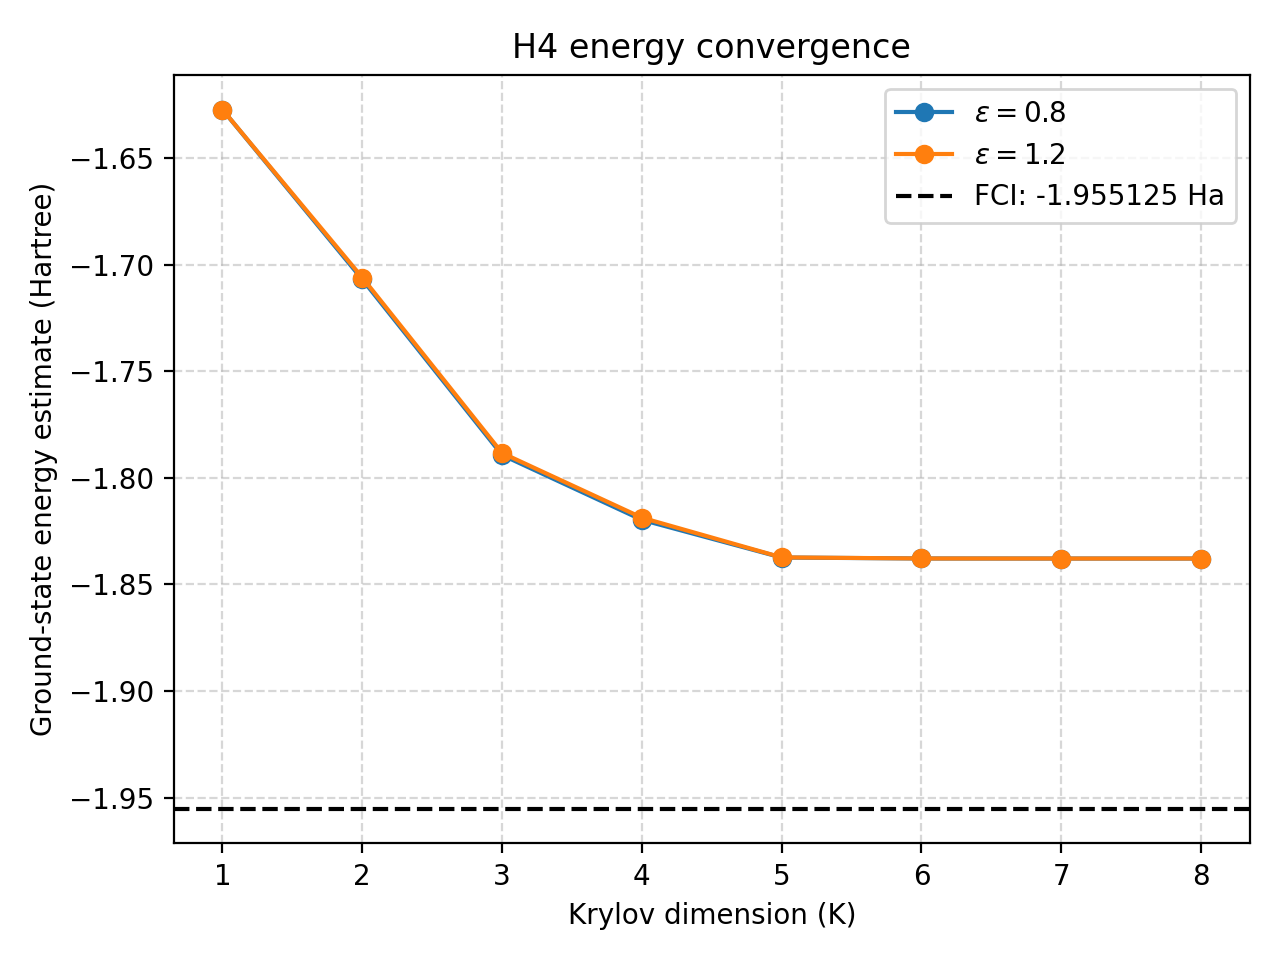
\includegraphics[width=0.87\linewidth]{../output/energy_convergence.png}
\caption{Physical projected energies in the saved H\(_4\) example.
The horizontal line is the fixed-sector FCI benchmark.}
\label{fig:energy}
\end{figure}

\begin{figure}[ht]
\centering
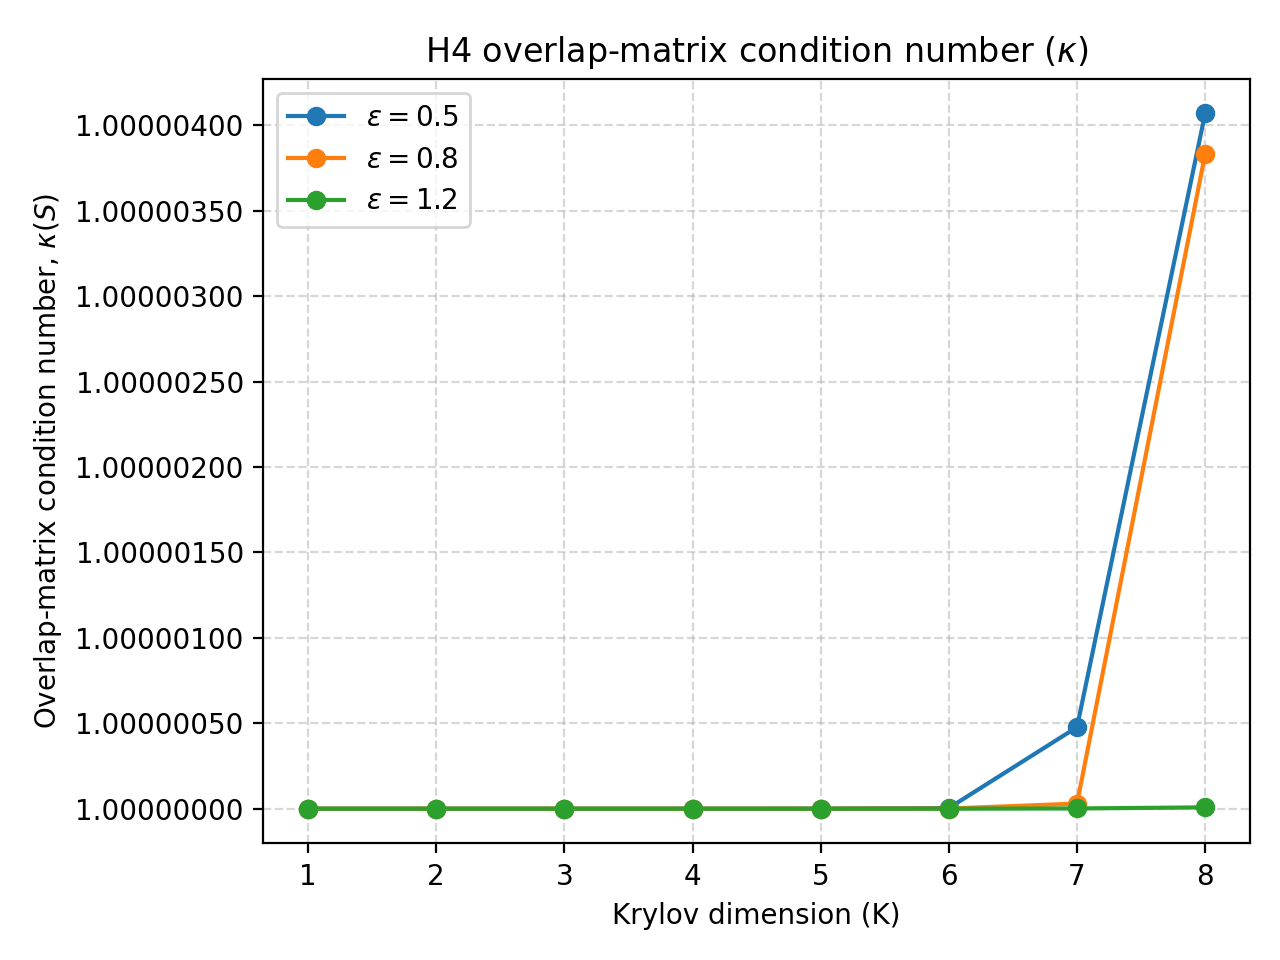
\includegraphics[width=0.87\linewidth]{../output/condition_number.png}
\caption{Actual overlap condition number
\(\kappa(S)=s_{\max}/s_{\min}\), without excess scaling.
The apparent late-step rise is small in absolute terms.}
\label{fig:condition}
\end{figure}

\clearpage

\section{Numerical accuracy and interpretation}

Three-term Lanczos produces orthogonal states in exact arithmetic.
This implementation reconstructs later states from Chebyshev
coefficient lists in floating-point arithmetic and does not
reorthogonalize them.  For the H\(_4\) example the later
coefficients can become very large while their polynomial sum
produces a unit vector; cancellation leaves small overlaps with
earlier states.  Normalization controls the state length, not those
overlaps.  Thus \(\kappa(S)\) slightly above one is a meaningful
diagnostic, but the plotted values near \(1.00000\) do not indicate
a nearly singular basis.  Near recurrence breakdown, the final
digits of \(\beta\), energy, and \(\kappa(S)\) are sensitive to the
floating-point execution path.

The moment identity in Eq.~\eqref{eq:beta-moment} relies on
orthogonality.  In exact-mode code, Eq.~\eqref{eq:exact-ritz}
also assumes \(S=I\), even when floating-point reconstruction
gives \(S\) a small deviation from identity.  Finite-shot mode
instead solves the retained generalized problem.  A stricter
orthogonal basis would require reorthogonalization, a more stable
state recurrence, or higher precision; those are not part of the
current \texttt{run()} path.

Dense diagonalization, generic dense state preparation, and exact
dense time-evolution matrices scale exponentially with qubit count.
The implementation is therefore an exact small-system study of
the measurement and recurrence formulas, not an efficient
large-system quantum circuit construction.

\appendix
\section{Optional collected-expression verification}
\label{app:collected}

\texttt{collected\_expressions()} is a separate high-precision
reference calculation.  It is not called by \texttt{run()} and
does not generate its circuit measurements.  Let the monic
Lanczos polynomials in \(x\) satisfy
\begin{equation}
 p_0(x)=1,\quad
 p_1(x)=x-\alpha_0,\quad
 p_{n+1}(x)=(x-\alpha_n)p_n(x)-\beta_n^2p_{n-1}(x).
 \label{eq:monic}
\end{equation}
With \(B_n=\prod_{j=1}^{n}\beta_j\), the ideal normalized state is
\(\ket{q_n}=p_n(X_\eps)\ket{\Phi_0}/B_n\).
Write \(p_n(x)^2=\sum_{p=0}^{2n}b_p x^p\).  Since
\(X_\eps=(U_\eps+U_\eps^\dagger)/2\) and \(U_\eps\) is unitary,
the coefficient of \(U_\eps^k\) in \(p_n(X_\eps)^2\), for
\(0\leq k\leq2n\), is
\begin{equation}
 a_k=\sum_{\substack{p\geq k\\p-k\ {\rm even}}}
 b_p\,2^{-p}
 \binom{p}{(p-k)/2}.
 \label{eq:unitary-coefficient}
\end{equation}
Because \(H\), \(X_\eps\), and \(U_\eps\) are functions of the
same Hermitian matrix and commute,
\begin{equation}
 \bra{q_n}H\ket{q_n}
 =\frac{
 a_0\bra{\Phi_0}H\ket{\Phi_0}
 +2\sum_{k=1}^{2n}a_k
 \operatorname{Re}\bra{\Phi_0}H U_\eps^k\ket{\Phi_0}}
 {B_n^2}.
 \label{eq:collected-energy}
\end{equation}
The helper recomputes the spectral recurrence and sine/cosine
values with \texttt{Decimal} arithmetic, expands the right side,
and checks it against the direct spectral expectation.  This
verifies algebra and cancellation in the collected expression;
its input Hamiltonian is still the floating-point matrix supplied
to the solver.

\section*{Source note}

This guide documents the code in \texttt{cqkud.py} and
\texttt{examples/h4.py}.  Its sine convention matches the local
\emph{OCQKUDSIN Mathematical implementation} reference.  The
related local \emph{OCQKU Step-by-Step Mathematical Implementation}
uses the divided-by-\(\eps\) operator described in Section~2.

\end{document}
